\subsection{Tutorien}

% TODO Der Begriff Tutorium ist hier recht eigenwillig genutzt. An den meisten anderen Unis versteht man unter "Tutorium" eher das, was hier "Praktikum" oder "Übung" ist, und dort ist dann "Praktikum" wieder was ganz anderes. Darauf könnte man kurz hinweisen.

% TODO dieser Abschnitt ist aus diverse Kapiteln zusammengeklebt und braucht dringend noch Aufräumung!

In diesem Abschnitt geht es um eure Tutorengruppen, die aus 2 Tutorengruppenleitern (Tutoren) sowie 10--15 Erstis bestehen und euch den Einstieg ins Studium erleichtern sollen.\\
Erfahrungsgem"a"s treten in der Anfangszeit einige Fragen auf. Oft wei"s man noch nicht genau, an wen man sich wenden sollte, oder kann den etwas bescheidenen Internetseiten der TU nicht die richtigen Informationen entlocken. In diesen F"allen sind die Tutoren die richtigen Ansprechpartner.\\

Ihr werden den Tutoren am Montag um ca. 15:00 Uhr zugeteilt. Dies geschieht am Ende der entsprechenden Veranstaltungen in den Räumen IZ 160 und IZ 161, in denen ihr euch dann (hoffentlich) befindet, je nach dem ob ihr Bachelor- oder Master-Studenten seid.

% NOTE: Hier war einiges redundant, außerdem nicht mehr aktuell. Habe großzügig auskommentiert, evtl. kann man das auch alles ganz löschen.

% Vom besonderen Interesse dürften dabei die allgemeine Einführung sein,
%sowie das Ersti-Begrüßung mit anschließenden Rundgang mit der
%Tutorengruppe.
%Dazu werden wir euch %nach dem Frühstück 
%Montag ab 15:00 Uhr in oder vor Raum IZ 160 studentische 
%Tutoren zuteilen,.
Mit diesen Tutoren werdet ihr direkt danach das Unigel"ande und Anderes erkunden.
Bei ihnen k"onnt ihr auch die ersten Fragen loswerden, wenn 
ihr nicht bei einem der beiden Beratungstermine davor wart, oder eure Fragen dort keinen Platz hatten.

%Die Einteilung findet nach den Begrüßungsveranstaltungen statt und erfolgt nach
%Bachelor und Master getrennt.
%Jedem Ersti soll in der Einf"uhrungswoche (s. Termine) eine Tutorengruppe zugeteilt werden. Damit auch ihr wisst, an wen ihr euch wenden k"onnt, solltet ihr diese Einteilung und das anschlie"sende %erste Treffen nicht verpassen!\\
%Dort habt ihr außerdem die M"oglichkeit in "uberschaubarer Runde andere Informatikstudenten des 1. Semesters kennen zu lernen, weitere Informationen zu euren Veranstaltungen und Dozenten zu %erhalten und das Campusgel"ande kennen zu lernen.\\

Scheut euch nicht, einen der Tutoren zu kontaktieren. Ihr k"onnt euch auch nachtr"aglich noch in eine Tutorengruppe einteilen lassen, da weitere Treffen geplant sind. Dazu schreibt bitte eine Mail an die Fachgruppe \nurl{fginfo@tu-bs.de} oder direkt an einen der Tutoren.\\

% TODO hier evtl. den Unterschied zwischen Tutor und Mentor erwähnen?

\end{multicols}
\ifpdf
Damit ihr auch ein paar Gesichter zuordnen k"onnt - gerade wenn ihr eventuell selbst noch keinen Tutor habt - sind hier Fotos einiger Tutoren abgebildet:

% TODO Bilder aktualisieren, angeben, ob der jenige Bachelors oder Masters betreut (ist ja nicht immer identisch damit, was man selbst gerade ist)
% NICHT als \paragraph, da das leider das Layout verhaut. Ist natürlich
% unschön ):
%Leider ist das ganze Layout etwas screwed
%Also ein alter Trick aus Web 1.0 Tagen\ldot.
%Layout Tabellen! Nicht schön, aber wenns sonst nicht geht\ldot.
\begin{center}
\begin{tabular}{ccc}
  { \textbf{Bachelor Tutoren}} \ \\ 
% \npicture[0.3\linewidth]
% {bilder/tutoren/kris.jpg}
% {Christoph\\ 3. Semester Master\\ \randomize{admin@keeg.de}}
% \ {
{
\npicture[0.3\linewidth]
{bilder/tutoren/dominik.jpg}
{Dominik\\2. Semester Master\\ \randomize{d.schuermann@tu-bs.de}}
}%\hfill
& \ 
%{\npicture[2.3\linewidth]
%{bilder/tutoren/franziska.jpg}
%{Franziska\\6. Semester Bachelor\\ \randomize{f.werk@tu-bs.de}}
%}%\\ \ \\
{\npicture[0.3\linewidth]
{bilder/tutoren/keno.jpg}
{Keno\\2. Semester Bachelor\\ \randomize{k.garlichs@tu-braunschweig.de}}
}
&
{
\npicture[0.3\linewidth]
{bilder/tutoren/hella.jpg}
{Hella\\ 1. Semester Master\\ \randomize{h-f.hoffmann@tu-bs.de}}}
 \\ \  \\
%\hfill
{\npicture[0.3\linewidth]
{bilder/tutoren/johannes.jpg}
{Johannes\\ 6. Semester Bachelor\\ \randomize{J.Starosta@tu-bs.de}}
}%& \ 
%\hfill
% {\npicture[0.3\linewidth]
% {bilder/tutoren/judith.jpg}
% {Judith\\ 5. Semester Bachelor\\ \randomize{judith.hilpert@web.de}}}\\
% \ \\
% \npicture[0.3\linewidth]
% {bilder/tutoren/marekd.jpg}
% {Marek\\ 1. Semester Master\\ \randomize{m.drogon@tu-bs.de}}
% &  %\hfill
% {
% \npicture[0.3\linewidth]
% {bilder/tutoren/sebastian.jpeg}
% {Sebastian\\ 7. Semester Bachelor\\ \randomize{se.busse@tu-bs.de}}}
&{
\npicture[0.3\linewidth]%{}
{bilder/tutoren/serj}
{Serj\\ 1. Semester Master\\\randomize{s.dechand@tu-bs.de }}}
%\par \ \par  
%\end{tabular}
%
%\begin{center}
%  \begin{tabular}{ccc}
 %    { \npicture[0.3\linewidth]%{}
 % {bilder/tutoren/christina}
 % {Christina\\ 5. Semester Bachelor\\\randomize{c.eberth@tu-bs.de}}}
&%{
%\npicture[0.3\linewidth]%{}
%{bilder/tutoren/viktor}
%{Viktor Richert\\ 4. Semester Bachelor\\%}%\\ 5. Semester Bachelor\\
%\randomize{InformatikWiki@gmx.de}}%.eberth@tu-bs.de }
% }&{
%  \npicture[0.3\linewidth]%{}
%  {bilder/tutoren/dummy}
%  {Christoph\\ 5. Semester Bachelor\\ \randomize{christoph.harburg@web.de}}
% }\\
{\npicture[0.3\linewidth]%{}
{bilder/tutoren/joko}
{Jonathan\\ 6. Semester Bachelor \\
\randomize{j.koscielny@tu-bs.de}}
}\end{tabular}\end{center}
%\begin{left}
\newpage
{ \textbf{Master Tutoren}}\\
\begin{center}
\begin{tabular}{ccc}
% NICHT als \paragraph, da das leider das Layout verhaut. Ist natürlich
% unschön ):
\npicture[0.3\linewidth]
{bilder/tutoren/martinw.jpg}
{Martin\\ 4. Semester Master\\ \randomize{m.wegner@tu-bs.de}}
&
{ 
\npicture[0.3\linewidth]
{bilder/tutoren/jan.jpg}
{Jan\\ 4. Semester Master\\ \randomize{jhkluth@gmx.de}}
}&%\\
%\hfill %\par \ \par

%{
%\npicture[0.3\linewidth]
%{bilder/tutoren/henning.jpg}
%{Henning\\ 5. Semester Master\\ \randomize{h.guenther@tu-bs.de}}
%}&
{ 
\npicture[0.3\linewidth]
{bilder/tutoren/sophia}
{Sophia\\ 2. Semester Master\\
\randomize{s.scholtka@tu-braunschweig.de}}
}\\
{\npicture[0.3\linewidth]
{bilder/tutoren/brian.jpg}
{Brian\\ 4. Semester Master\\ \randomize{b.schimmel@tu-bs.de}}
}&
%\hfill
{\npicture[0.3\linewidth]
{bilder/tutoren/hashier.jpg}%Christopher Lössl < c.loessl@tu-bs.de>
{Chris \\3. Semester Master\\ \randomize{c.loessl@tu-bs.de}}
}%&
%{\npicture[0.3\linewidth]
%{bilder/tutoren/dummy}
%{Till \\  2. Semester Master\\\randomize{t.lorentze@tu-bs.de}}
%}
%\npicture[0.3\linewidth]
%{bilder/tutoren/stephan.jpg}
%{Stephan\\ 5. Semester Master\\ stephan.friedrichs@tu-bs.de}


  \end{tabular}
  
\end{center}
    \begin{center}
          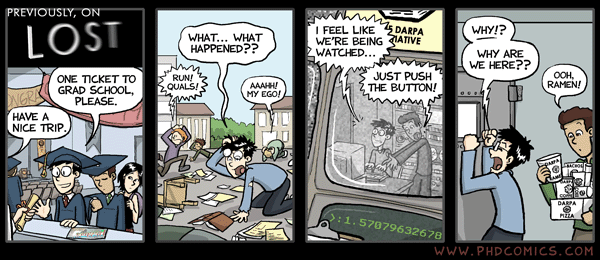
\includegraphics[width=\linewidth]
	  {bilder/comics/phd092706s.png}    \end{center}

\else
In der Druckfassung wären hier die Tutoren mit Emailadresse und Foto aufgelistet. Um die Privatspäre der Tutoren zu schützen, stehen diese jedoch nicht direkt hier in der Onlinefassung.
\fi

\begin{multicols}{2}
%%% Local Variables: 
%%% mode: latex
%%% TeX-master: "../../1-te"
%%% End: 
